\documentclass{standalone}
% tikz-feynhand: e+ e- annihilation into a photon and a fermion pair.
% (feynhand provides \vertex and \propag; there is no \diagram command.)
\usepackage{tikz-feynhand}
\begin{document}
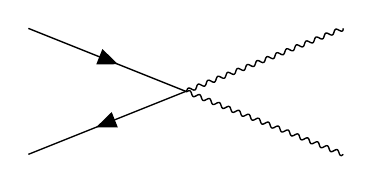
\begin{tikzpicture}
\begin{feynhand}
\vertex (i1) at (-2, 0.8);
\vertex (i2) at (-2,-0.8);
\vertex (m)  at ( 0, 0);
\vertex (f1) at ( 2, 0.8);
\vertex (f2) at ( 2,-0.8);
\propag[fermion] (i1) to (m);
\propag[anti fermion] (i2) to (m);
\propag[photon] (m) to (f1);
\propag[photon] (m) to (f2);
\end{feynhand}
\end{tikzpicture}
\end{document}
